\section{Descriptive statistics of vulnerable resources}
\subsection{Country overview}
\autoref{fig:map} presents geographic distribution of vulnerable resources. In highlighted countries, we detected at least one vulnerable server while the size of each circle is proportional to their number. We discovered vulnerable servers in 125 countries across the globe including all the countries in Europe, North America and a vast majority of countries in Asia, South America, Australia and Oceania. Relatively low number of vulnerable servers in the African region can be explained by low number of total DNS servers in the area \footnote{\url{https://labs.ripe.net/Members/emileaben/dns-root-server-transparency}}. \michal{We can probably get a better reference here}

The vast majority of vulnerable servers are located in Japan (716151), US (6442), South Korea (2922), Turkey (2701), Brazil (2080), Germany (1209), Taiwan (1135) and Canada (1047). 

\begin{figure}[!hbt]
\centering
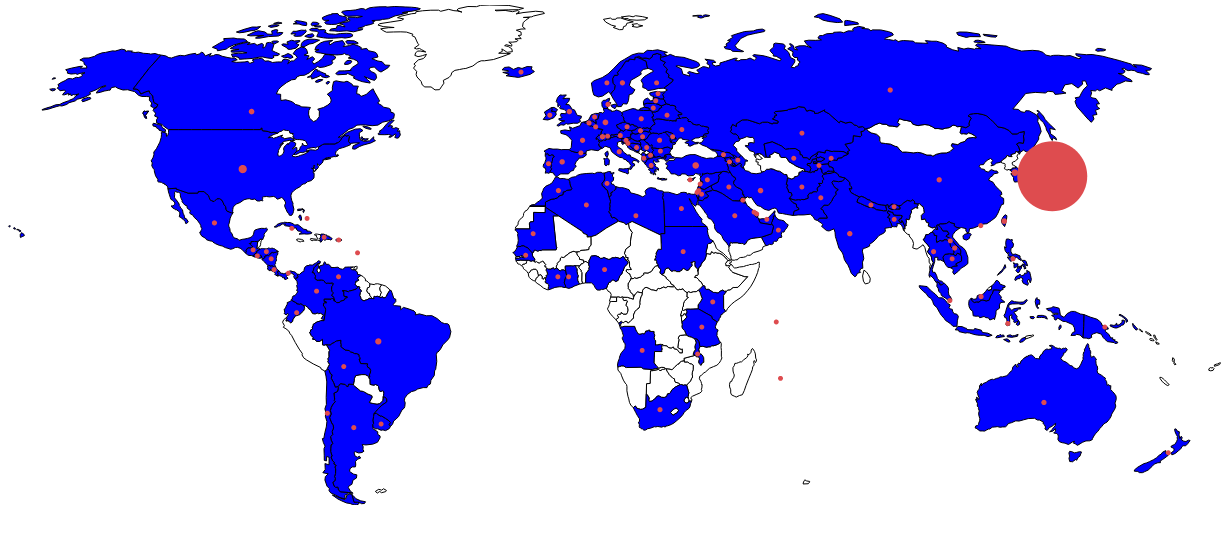
\includegraphics[width=1\columnwidth]{map.png}
\caption{Countries}
\label{fig:map}
\end{figure}

\begin{figure}[!hbt]
\centering
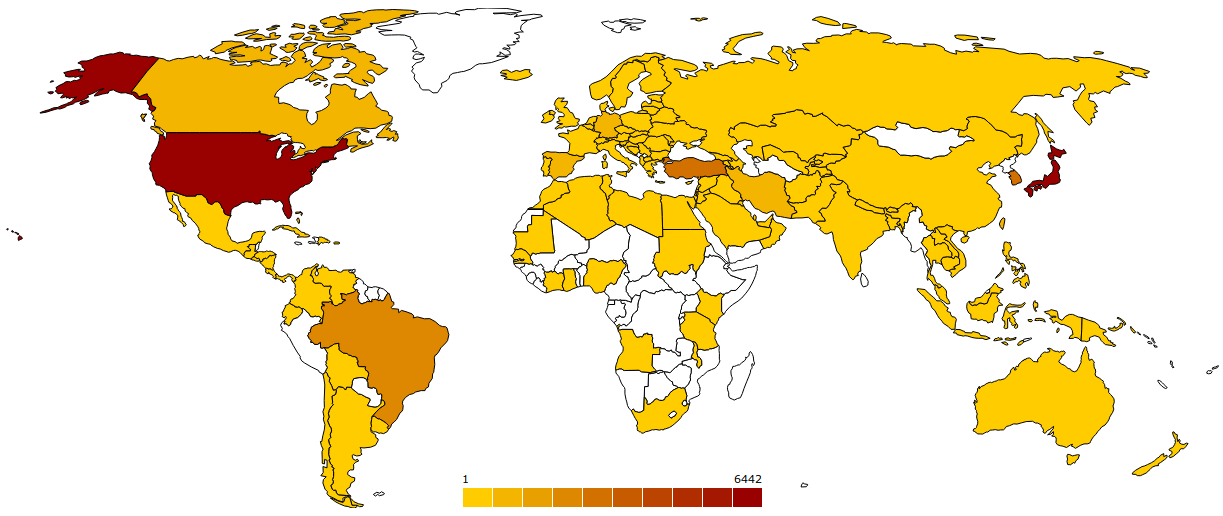
\includegraphics[width=1\columnwidth]{heatmap.png}
\caption{Heatmap - Japan aligned with the US}
\label{fig:heatmap}
\end{figure}

\subsection{Per-AS statistics}
We continue by investigating distribution of vulnerable resources across different Autonomous Systems (AS). \autoref{fig:ip_pie} shows 
\begin{figure}[!hbt]
\centering
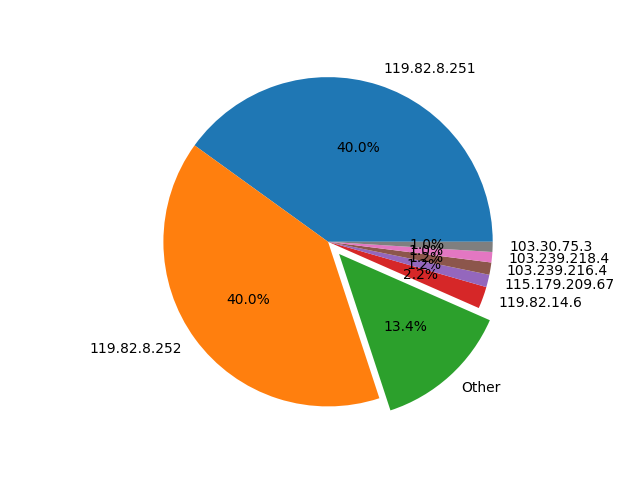
\includegraphics[width=.8\columnwidth]{ip_pie.png}
\caption{IP addresses}
\label{fig:ip_pie}
\end{figure}

\begin{figure}[!hbt]
\centering
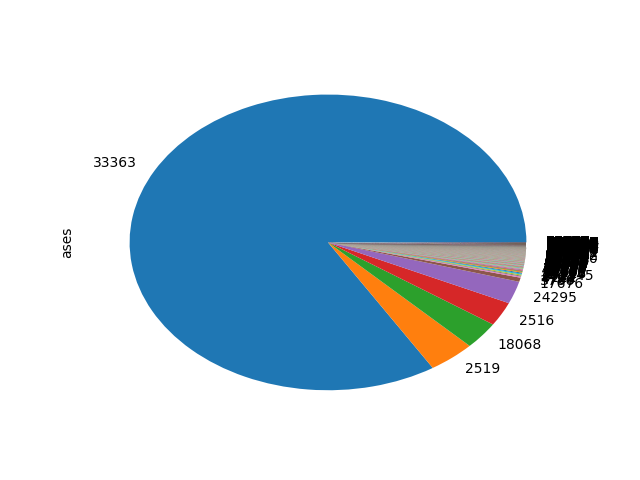
\includegraphics[width=.8\columnwidth]{ip_as_pie.png}
\caption{AS}
\label{fig:ip_as_pie}
\end{figure}

\subsection{Per-CERT statistics}
\subsection{Per-TLD statistics}
\subsection{Popularity of affected domains}
